\newpage
\section{Database System Concepts and Architecture}

% Definizioni sui modelli
\subsection{Definizioni sui modelli}

Le definizioni di base da sapere sono:

\begin{itemize}
	\item \hl{Data Model}: insieme di \textbf{concetti che descrivono struttura, operazioni e vincoli} applicati al DB
	
	\item \hl{Data Model Structure and Constraints}: abbiamo dei \textbf{costrutti che definiscono come collegare gli elementi} definiti da: entità, record e tabella

	\item \hl{Data Model Operation}: di base (\textbf{CRUD}) o definite dall'utente

	\item \hl{modello dal concettuale}: di \textbf{alto livello} e semantico
	
	\item \hl{modello fisico}: di basso livello, definisce \textbf{come i dati sono salvati}
	
	\item \hl{modello implementativo}: usati nel DBMS 
	
	\item \hl{modello autodescrivente}: basati su XML 

\end{itemize}


% Definizioni fondamentali
\subsection{Definizioni fondamentali}

\begin{itemize}
	\item \hl{DataBase schema}: descrizione del database in termini di struttura, tipo dati e vincoli
	
	\item \hl{schema diagram}: \textbf{visione rappresentativa} del DB schema
	
	
\begin{figure}[H]
\centering
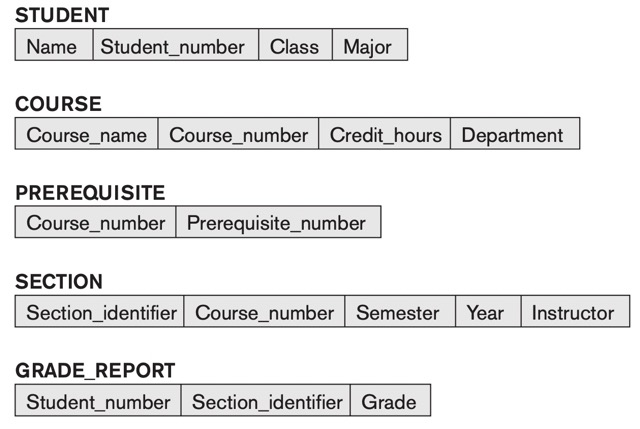
\includegraphics[scale=0.4]{schcon.jpeg}
\caption{Schema diagram} 
\label{schcon}
\end{figure}
	
	
	\item \hl{schema construct}: insieme tra \textbf{schema e dati} dei DB


	\item \hl{database state}: \textbf{snapshot} in istante t del DB, si definisce quindi ai suoi contenuti
	
	\item \hl{valid state}: si definisce funzionante se il suo contenuto \textbf{soddisfa i vincoli} per quello schema
	
	\item \hl{data dictioraty}: insieme per salvare schema e altre info 
\end{itemize}


% Schema
\subsection{Schema}

Possiamo avere 3 \hl{livelli di schema}:

\begin{enumerate}
	\item \textbf{interno (fisico)}: come i dati devono essere salvati e come posso accederci
	\item \textbf{concettuale}
	\item \textbf{esterno}: per descrivere le view dell'utente
\end{enumerate}


\hl{Per passare da uno schema ad un altro} ho bisogno di un \hl{mapping} per capire a cosa corrisponde un elemento. Avremo:

\begin{itemize}
	\item \hl{logic data independence}: se voglio \textbf{cambiare lo schema concettuale} senza cambiare quello fisico
	\item \hl{physical}: devo \textbf{cambiare lo schema fisico} senza cambiare quello concettuale
\end{itemize}


% Tipologie di DBMS
\subsection{Tipologie di DBMS}

Possiamo avere più tipologie di DBMS:

\begin{itemize}
	\item \hl{centralized}: dove abbiamo tutta l'\textbf{elaborazione su un unico nodo}
	\item \hl{2-tier}: si specializza in termini di server per ogni blocco di funzionalità che devo offrire
	\item \hl{cliets}: per far accedere gli utenti
	\item \hl{DBMS server}: per eseguiire query e transazioni tramite API
\end{itemize}

